
\makeatletter

\def\@makechapterhead#1{%
  \vspace*{50\p@}%
  {\parindent \z@ \raggedright \normalfont
    \ifnum \c@secnumdepth >\m@ne
      \if@mainmatter
        \huge\bfseries Appendix\space \thechapter
       \par\nobreak
        \vskip 20\p@
      \fi
    \fi
    \interlinepenalty\@M
    \Huge \bfseries #1 \par\nobreak
    \vskip 40\p@
  }}

\c@tocdepth=1
\renewcommand\thesection{\@Alph\thechapter.\@arabic\c@section}

\def\@chapter[#1]#2{\ifnum \c@secnumdepth >\m@ne
                       \if@mainmatter
                         \refstepcounter{chapter}%
                         \typeout{\@chapapp\space\thechapter.}%
                         \addcontentsline{toc}{chapter}%
                                   {\protect\numberline{}
                         Appendix 1: #1}%
                       \else
                         \addcontentsline{toc}{chapter}{#1}%
                       \fi
                    \else
                      \addcontentsline{toc}{chapter}{#1}%
                    \fi
                    \chaptermark{#1}%
                    \addtocontents{lof}{\protect\addvspace{10\p@}}%
                    \addtocontents{lot}{\protect\addvspace{10\p@}}%
                    \if@twocolumn
                      \@topnewpage[\@makechapterhead{#2}]%
                    \else
                      \@makechapterhead{#2}%
                      \@afterheading
                    \fi}

\makeatother

\setcounter{chapter}{0}
\chapter[Practical Verification of the Conditions.....]{Practical Verification of the Conditions $(\mathbb{R} - N. D.)$ and $(\mathbb{C}- N. D.)$ when $n = 2$ and Remarks on the General Case.}


Let\pageoriginale $q = (q_{\alpha})_{\alpha = 1, 2}$ be a homogeneous polynomial mapping of degree $k$ on $\mathbb{R}^{3}$ with values in $\mathbb{R}^{2}$. Given a system of coordinates $(\widetilde{e}_{1}, \widetilde{e}_{2}, \widetilde{e}_{3})$ of $\mathbb{R}^{3}$, we set for $\widetilde{\xi} \epsilon \mathbb{R}^{3}$
\begin{equation*}
\widetilde{\xi} = \xi_{1} \widetilde{e}_{1} + \xi_{2}\widetilde{e}_{2} + \xi_{3} \widetilde{e}_{3},\tag{A.1}\label{chap5-eqA.1}
\end{equation*}
where $\xi_{1}, \xi_{2}, \xi_{3} \epsilon \mathbb{R}$ and define
\begin{equation*}
{\widetilde{\xi}}' = \xi_{1} \widetilde{e}_{1} + \xi_{2} \widetilde{e}_{2},\tag{A.2}\label{chap5-eqA.2}
\end{equation*}
so that 
\begin{equation*}
\widetilde{\xi} = {\widetilde{\xi}}' + \xi_{3} \widetilde{e}_{3}.\tag{A.3}\label{chap5-eqA.3}
\end{equation*}

With these notations, each polynomial $q_{\alpha}$ is expressed as
\begin{equation*}
q_{\alpha}(\widetilde{\xi}) = \sum\limits_{s=0}^{k} a_{\alpha, s} (\widetilde{\xi}') \xi_{3}^{s}, \alpha = 1, 2\tag{A.4}\label{chap5-eqA.4}
\end{equation*}
where $a_{\alpha, s}$ is a homogeneous polynomial of degree $k - s$. Now, note that either the condition $(\mathbb{R} - N. D.)$ fails of $\widetilde{e}_{3}$ can be chosen so that $q_{1}(\widetilde{e}_{3}) \neq 0$ and $q_{2}(\widetilde{e}_{3}) \neq 0$. Indeed, this is possible unless $q_{1}q_{2} = 0$, namely $q_{1} \equiv 0$ or $q_{2} \equiv 0$. But, in this case, the condition $(\mathbb{R}-N.D.)$ is not satisfied by $q$.

With this choice of $\widetilde{e}_{3}$, one has
\begin{equation*}
a_{\alpha, k} = q_{\alpha} (\widetilde{e}_{3}) \neq 0, \alpha = 1, 2.\tag{A.5}\label{chap5-eqA.5}
\end{equation*}

Then, $q(\widetilde{\xi}) = 0$ if and only if the two polynomials in $\xi_{3}$ of degree {\em exactly}\pageoriginale $k$
\begin{equation*}
\xi_{3} \to q_{\alpha} (\widetilde{\xi}' + \xi_{3} \widetilde{e}_{3}), \alpha = 1, 2,\tag{A.6}\label{chap5-eqA.6}
\end{equation*}
have a common real root for the prescribed value $\widetilde{\xi}'$. As the leading coefficients $a_{1, k}$ and $a_{2, k}$ are nonzero, the resultant $\mathbb{R}(\widetilde{\xi}')$ of these two polynomials vanishes for this values of $\widetilde{\xi}'$.

We examine the converse of this result. First, the resultant $\mathbb{R}$ can identically vanish: It is well - known that this happens if and only if $q_{1}$ and $q_{2}$ have a nonconstant (homogeneous) common factor. Let us then write
$$
q_{1} = rp_{1}, q_{2} = rp_{2}
$$
with $p_{1}$ and $p_{2}$ relatively prime, deg $r \geq 1$. If $r$ vanishes at some point $\widetilde{\xi} \epsilon \mathbb{R}^{3} - \{0\}$, one has
$$
q_{\alpha} (\widetilde{\xi}) = 0, \alpha = 1, 2,
$$
and
$$
Dq_{\alpha}(\widetilde{\xi}) = P_{\alpha}(\widetilde{\xi}) Dr(\widetilde{\xi}), \alpha = 1, 2.
$$

Thus, $\Ker Dq(\widetilde{\xi}) \supset Ker Dr(\widetilde{\xi})$ whose dimension is $\geq 2$ and $q$ does not satisfy the condition $(\mathbb{R}-N.D.)$.

If $r$ does not vanish in $\mathbb{R}^{3} - \{0\}$ (note that $r$ {\em does} vanish in $\mathbb{C}^{3} - \{0\}$ from Hilbert's zero theorem), there is no line in the zero set of $q$ in $\mathbb{R}^{3}$ which is in the zero set of $r$ and we can replace $q_{1}$ and $q_{2}$ by $p_{1}$ and $p_{2}$. From now, on, we can then assume that $q_{1}$ and $q_{2}$ are relatively prime, so that
$$
\mathscr{R} \nequiv 0.
$$

It\pageoriginale can be shown by simple arguments that $\mathscr{R}$ is a homogeneous polynomial of degree $k^{2}$ (see e.g. \cite{16, 18}). Its zero set in $\mathbb{R} \widetilde{e}_{1} \oplus \mathbb{R} \widetilde{e}_{2}$ then consists of a finite number of lines $(\leq k^{2})$ through the origin and the same result is true in the space $\mathbb{C} \widetilde{e}_{1} \oplus \mathbb{C} \widetilde{e}_{2}$ (of course, in this case, the lines in the zero set of $\mathscr{R}$ are {\em complex} ones). For the sake of convenience, we shall denote by $\mathbb{K}$ either field $\mathbb{R}$ of $\mathbb{C}$. Given a point $\widetilde{\xi}' \epsilon \mathbb{K} \widetilde{e}_{1} \oplus \mathbb{K} \widetilde{e}_{2}$ such that $\mathscr{R} (\widetilde{\xi}') = 0$, there is a finite number $(\geq 1)$ of values $\xi_{3} \epsilon \mathbb{C}$ such that $q(\widetilde{\xi}' + \xi_{3} \widetilde{e}_{3}) = 0$: These values are the common roots in $\mathbb{C}$ of the two polynomials (\ref{chap5-eqA.6}) (hence their number is finite). It follows that, above each $\mathbb{K}$-line in the zero set of $\mathscr{R}$ in $\mathbb{K} \widetilde{e}_{1} \oplus \mathbb{K} \widetilde{e}_{2}$, there is a finite number of $\mathbb{K}$-lines in the zero set of $q$. However, when $\mathbb{K} = \mathbb{R}$, there lines may not lie in $\mathbb{R}^{3}$ since, for a given $\widetilde{\xi}' \epsilon \mathbb{R} \widetilde{e}_{1} \oplus \mathbb{R} \widetilde{e}_{2}$ in the zero set of $\mathscr{R}$, some corresponding values $\xi_{3}$ such that $q(\widetilde{\xi}' + \xi_{3}\widetilde{e}_{3}) = 0$ may belong to $\mathbb{C} \backslash \mathbb{R}$. But this happens in ``almost'' no system $(\widetilde{e}_{1}, \widetilde{e}_{2}, \widetilde{e}_{3})$. To see this, let us consider an arbitrary change of $\widetilde{e}_{3}$ into $\widetilde{e}_{3}^{*}$ such that $(\widetilde{e}_{1}, \widetilde{e}_{2}, \widetilde{e}_{3}^{*})$ is a basis of $\mathbb{R}^{3}$. The coordinates $(\xi_{1}^{*}, \xi_{2}^{*}, \xi_{3}^{*})$ of any point $\widetilde{\xi} \epsilon \mathbb{R}^{3}$ in this basis are given by
\begin{equation*}
\begin{bmatrix}
\xi_{1}^{*}\\
\xi_{1}^{*}\\
\xi_{31}^{*}
\end{bmatrix}
=
\begin{bmatrix}
1 & 0 & a\\
0 & 1 & b\\
0 & 0 & c
\end{bmatrix}
\begin{bmatrix}
\xi_{1}\\
\xi_{2}\\
\xi_{3}
\end{bmatrix}
,\tag{A.7}\label{chap5-eqA.7}
\end{equation*}
where $(\xi_{1}, \xi_{2}, \xi_{3})$ are the coordinates of $\widetilde{\xi}$ in the basis $(\widetilde{e}_{1}, \widetilde{e}_{2}, \widetilde{e}_{3})$ and the coefficients $a$, $b$ and $c$ are real with $c \neq 0$. Of course, $(\widetilde{e}_{1}, \widetilde{e}_{2}, \widetilde{e}_{3})$\pageoriginale and $(\widetilde{e}_{1}, \widetilde{e}_{2}, \widetilde{e}_{3}^{*})$ are also bases in $\mathbb{C}^{3}$ and the change of coordinates is still given by (\ref{chap5-eqA.7}).

Let the $\mathbb{C}$-lines in the zero set of $q$ in $\mathbb{C}^{3}$ be generated by the nonzero vectors $\widetilde{\xi}_{1}, \cdots, \widetilde{\xi}_{\nu}$ with $\nu \leq k^{2}$ from Bezout's theorem. Denote by $(\xi_{j1}, \xi_{j2}, \xi_{j3})$ and $(\xi_{j1}^{*}, \xi_{j2}^{*}, \xi_{j3}^{*})$ the components of $\widetilde{\xi}_{j}$, $1 \leq j \leq \nu$, in the bases $(\widetilde{e}_{1}, \widetilde{e}_{2}, \widetilde{e}_{3})$ and $(\widetilde{e}_{1}, \widetilde{e}_{2}, \widetilde{e}_{3}^{*})$ respectively. For a fixed index $1 \leq j \leq \nu$, the first two components $\xi_{j1}^{*}$ and $\xi_{j2}^{*}$ will have the sasme argument if and only if (agreeing that 0 has  the same argument as any complex number)
\begin{align*}
(Re \xi_{j1} Im \xi_{j2} - Re \xi_{j2} Im \xi_{j1}) & + a(Re \xi_{j3} Im \xi_{j2} - Re \xi_{j2} Im \xi_{j3}) + \\
& + b(Re \xi_{j1} Im \xi_{j3} - Re \xi_{j3} Im \xi_{j1}) = 0
\end{align*}

In other words, if $\xi_{j1}, \xi_{j2}$ {\em and} $\xi_{j3}$ do not have the same argument, the above equality holds for $a$ and $b$ in a one-dimensional affine manifold of $\mathbb{R}^{2}$ while, from (\ref{chap5-eqA.7}), if $\xi_{j1}, \xi_{j2}$ and $\xi_{j3}$ have the same argument, the three components $\xi_{j1}^{*}, \xi_{j2}^{*}$ and $\xi_{j3}^{*}$ also have the same argument. To sum up, for $a$ and $b$ outside the union of a finite number $\leq \nu$ of one-dimensional affine manifolds in $\mathbb{R}^{2}$, the following property holds: For any $1 \leq j \leq \nu$, the two components $\xi_{j1}^{*}$ and $\xi_{j2}^{*}$ have the same argument if and only if $\xi_{j1}^{*}, \xi_{j2}^{*}$ {\em and} $\xi_{j3}^{*}$ have the same argument.

Now, let
$$
\widetilde{\xi} = \xi_{1}^{*} \widetilde{e}_{1} + \xi_{2}^{*} \widetilde{e}_{2} + \xi_{3}^{*} \widetilde{e}_{3}^{*},
$$
be\pageoriginale a nonzero element in the zero set of $q$ in $\mathbb{C}^{3}$ with $\xi_{1}^{*}, \xi_{2}^{*} \epsilon \mathbb{R}$. One has
$$
\widetilde{\xi} = \lambda \widetilde{\xi}_{j},
$$ 
for some $\lambda \epsilon \mathbb{C} - \{0\}$ and some $1 \leq j \leq \nu$. Thus $\xi_{1}^{*} = \lambda \xi_{j1}^{*}$, $\xi_{2}^{*} = \lambda \xi_{j2}^{*}$ and $\xi_{3}^{*} = \lambda \xi_{j3}^{*}$. As $\xi_{1}^{*}$ and $\xi_{2}^{*}$ are real by hypothesis, $\xi_{j1}^{*}$ and $\xi_{j2}^{*}$ have the same argument (namely, -Arg $\lambda$). Hence Arg $\xi_{j3}^{*} = -Arg \lambda$ too and it follows that $\xi_{3}^{*}$ is real.

Thus, by simply modifying $\widetilde{e}_{3}$, one can assume that above each $\mathbb{R}$-line in the zero set of $\mathscr{R}$ in $\mathbb{R}\widetilde{e}_{1} \oplus \mathbb{R} \widetilde{e}_{2}$, all the corresponding $\mathbb{R}$-lines in the zero set of $q$ in $\mathbb{C}^{3}$ lie in $\mathbb{R}^{3}$ (an equivalent way of saying that for every $\widetilde{\xi}' \epsilon \mathbb{R} e_{1} \oplus \mathbb{R} e_{2}$ such that $\mathscr{R}(\widetilde{\xi}') = 0$, all the solutions $\xi_{3} \epsilon \mathbb{C}$ of the equation $q(\widetilde{\xi}' + \xi_{3} \widetilde{e}_{3}) = 0$ are {\em real}). From the above proof, this property is unchanged by an arbitrarily small change of the vector $\widetilde{e}_{3}$. Of course, above a given $\mathbb{R}$-line in the zero set of $\mathscr{R}$ in $\mathbb{R} \widetilde{e}_{1} \oplus \mathbb{R} \widetilde{e}_{2}$ may lie several $\mathbb{R}$-lines in the zero set of $q$ in $\mathbb{R}^{3}$. Again, this happens in exceptional cases only. Indeed, the $\mathbb{R}$-lines in the zero set of $\mathscr{R}$ are the projections along $\widetilde{e}_{3}$ of the lines in the zero set of $q$. By slightly changing $\widetilde{e}_{3}$ and since there are only finitely many $\mathbb{R}$-lines in the zero set of $q$ in $\mathbb{R}^{3}$, we can manage so that the lines in the zero set of $q$ and the lines in the zero set of $\mathscr{R}$ are in one-to-one correspondence. We leave it to the reader to given a rigorous proof of this result, exemplified on Figure A.1 below: Given a basis $(\widetilde{e}_{1}, \widetilde{e}_{2}, \widetilde{e}_{3})$\pageoriginale of $\mathbb{R}^{3}$ and a finite number of lines in $\mathbb{R}^{3}$ which project onto the same line of the plane $\mathbb{R}\widetilde{e}_{1} \oplus \mathbb{R} \widetilde{e}_{2}$ along $\widetilde{e}_{3}$, any change of $\widetilde{e}_{3}$ into a non-collinear vector is so that the new projection onto $\mathbb{R} \widetilde{e}_{1} \oplus \mathbb{R} \widetilde{e}_{2}$ along $\widetilde{e}_{3}$ transforms these lines into the same number of {\em distinct} lines of the plane $\mathbb{R} \widetilde{e}_{1} \oplus \mathbb{R} \widetilde{e}_{2}$.

\begin{alphremark}\label{app-1-remA.1}
Of course, each change of the vector $\widetilde{e}_{3}$ {\em modifies} the polynomial $\mathscr{R}$, which is the reason why the above properties can be established.
\end{alphremark}

\renewcommand{\thefigure}{\Alph{section}.\arabic{figure}}
\setcounter{section}{1}
\setcounter{figure}{0}
\begin{figure}[H]
\centering
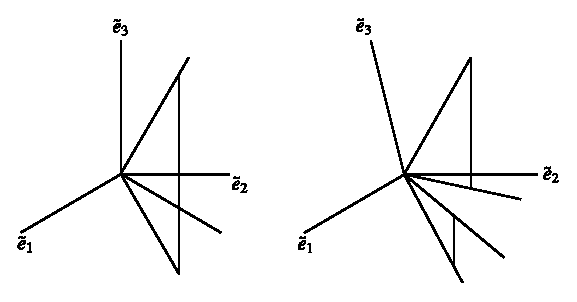
\includegraphics{figure/fig76-A-1.eps}
\caption{}
\end{figure}

The basis $(\widetilde{e}_{1}, \widetilde{e}_{2}, \widetilde{e}_{3})$ being now fixed so that the previous properties hold, we are in position to give a characterization of the condition $(\mathbb{R}-N.D.)$. First, as $\mathscr{R} \nequiv 0$ and by a suitable choice of $\widetilde{e}_{2}$ {\em without modifying} $\mathbb{R} \widetilde{e}_{1} \oplus \mathbb{R}\widetilde{e}_{2}$ (so that the definition of $\mathscr{R}$ is not affected) we may assume $\mathscr{R}(\widetilde{e}_{2}) \neq 0$. As $\mathscr{R}$ is homogeneous of degree $k^{2}$, $\widetilde{\xi}' = 0$\pageoriginale is always in the zero set of $\mathscr{R}$. From (\ref{chap5-eqA.5}), this value corresponds with the value $\widetilde{\xi} = 0$ in the zero set of $q$, a solution in which we have no interest. All then amounts to finding the nonzero solutions of $\mathscr{R}(\widetilde{\xi}') = 0$. By our choice of $e_{2}$, none of them is of the form $\xi_{2} \widetilde{e}_{2}$ (i.e. $\xi_{1} = 0$) and, after dividing by $\xi_{1}^{k^{2}} \neq 0$
$$
\mathscr{R}(\widetilde{\xi}') = 0 \leftrightarrow \mathscr{R}(\widetilde{e}_{1} + \frac{\xi_{2}}{\xi_{1}} \widetilde{e}_{2}) = 0
$$    

Setting $\tau = \xi_{2} | \xi_{1}$, each real root of the polynomial
\begin{equation*}
a(\tau) = \mathscr{R}(\widetilde{e}_{1} + \tau \widetilde{e}_{2}) = 0,\tag{A.8}\label{chap5-eqA.8}
\end{equation*}
corresponds with one and only one real line in the zero set of $\mathscr{R}$ in $\mathscr{R} \widetilde{e}_{1} \oplus \mathscr{R} \widetilde{e}_{2}$ and hence with {\em one and only one line in the zero set of} $q$ in $\mathbb{R}^{3}$. Then, the condition $(\mathbb{R}-N.D.)$ is equivalent to assuming that {\em each real root of polynomial $a(\tau)$ is simple}. We only sketch the proof of this result (which uses the notion of multiplicity of intersection). For the sake of brevity, we shall refer to the real zero set of q (resp. $\mathscr{R}$) as being the zero set of $q$ (resp. $\mathscr{R}$) in $\mathbb{R}^{3}$ (resp. $\mathbb{R} \widetilde{e}_{1} \oplus \mathbb{R} \widetilde{e}_{2})$. Similar definitions will be used for the complex zero sets of $q$ and $\mathscr{R}$.

A real line $L_{\mathbb{R}}$ in the real zero set of $q$ (resp. $\mathscr{R}$) is than the intersection of one and only one complex line $L_{\mathbb{C}}$ in  the complex zero set of $q$ (resp. $\mathscr{R}$) with $\mathbb{R}^{3}$ (resp. $\mathbb{R} \widetilde{e}_{1} \oplus \mathbb{R} \widetilde{e}_{2}$). Actually, if
$$
L_{\mathbb{R}} = \mathbb{R} \widetilde{\xi}_{0} (resp. \mathbb{R} \widetilde{\xi}'_{0}),
$$
then\pageoriginale
$$
L_{\mathbb{C}} = \mathbb{C} \widetilde{\xi}_{0} (resp. \mathbb{C} \widetilde{\xi}'_{0}).
$$

The line $L_{\mathbb{C}}$ will be called the complex extension of $L_{\mathbb{R}}$. From our previous results, above the extension $L_{\mathbb{C}}$ of a given line $L_{\mathbb{R}}$ in  the real zero set of $\mathscr{R}$ lines exactly one $\mathbb{C}$-line in the complex zero set of $q$ (whose intersection with $\mathbb{R}^{3}$ is nothing but this one $\mathbb{R}$-line in the real zero set of $q$ above $L_{\mathbb{R}}$).

To each $\mathbb{C}$-line $L_{\mathbb{C}}$ in the complex zero set of $q$ is associated a {\em multiplicity}, called the {\em multiplicity of intersection} of the surface $q_{1}(\widetilde{\xi}) = 0$ and $q_{2}(\widetilde{\xi}) = 0$ along $L_{\mathbb{C}}$. The following result is true in general (cf. \cite{11}): The multiplicity of the root $\tau \epsilon \mathbb{C}$ of the polynomial $a(\tau)$ (\ref{chap5-eqA.8}) equals the number of $\mathbb{C}$-lines in the complex zero set of $q$ which lie above the $\mathbb{C}$-line
$$
\{\xi_{1} \widetilde{e}_{1} + \tau \xi_{1} \widetilde{e}_{2}, \xi_{1} \epsilon \mathbb{C}\},
$$
in the complex zero set of $\mathscr{R}$, {\em counted with multiplicity}. On the other hand, from the condition $(\mathbb{R}-N.D.)$, the multiplicity of the complex extension of any $\mathbb{R}$-line in the real zero set of $q$ happens to be {\em one}, which, from our choice of the basis $(\widetilde{e}_{1}, \widetilde{e}_{2}, \widetilde{e}_{3})$, proves the equivalence of the condition $(\mathbb{R}-N.D.)$ with the fact that each real root of the polynomial $a(\tau)$ (\ref{chap5-eqA.8}) is simple.

The condition $(\mathbb{C}-N.D.)$ also bears a similar characterization. Here, the basis $(\widetilde{e}_{1}, \widetilde{e}_{2}, \widetilde{e}_{3})$ must be taken so that the projection onto $\mathbb{C} \widetilde{e}_{1} \oplus \mathbb{C} \widetilde{e}_{2}$ of all the $\mathbb{C}$-lines in the complex zero set of $q$ are distinct.\pageoriginale If so, the same arguments of multiplicity show that the condition $(\mathbb{C}-N.D.)$ is equivalent\footnote{As very nonconstant homogeneous polynomial vanishes at nonzero points in $\mathbb{C}^{3}$, it is necessary that $q_{1}$ and $q_{2}$ be relatively prims for the condition $(\mathbb{C}-N.D.)$ to hold.}  to assuming that {\em each root of the polynomial} $a(\tau)$ (\ref{chap5-eqA.8}) {\em simple} (as a result, it has exactly $k^{2}$ distinct roots, each of them providing a different $\mathbb{C}$-line in the complex zero set of $q$). It follows that the condition $(\mathbb{C}-N.D.)$ amounts to assuming that the {\em discriminant} of $a(\tau)$ (\ref{chap5-eqA.8}) {\em is} $\neq 0$: It is a $(2k^{2} - 1) \times (2k^{2} - 1)$ determinant\footnote{A note by H. Gerber (Amer.Math. Monthly, 91(1984), pp.644-646) on reducing the size of determinants for calculating resultants may be applicable here.} whose coefficients are completely determined by the polynomials $q_{1}$ and $q_{2}$ and is then particularly simple to work out in practice.

In both cases, besides a criterion for checking the non-degeneracy condition, we have got a practical means of calculation of (approximations of) the $\mathbb{R}$-lines in the real zero set of $q$ by calculating (approximations of) the real roots of the polynomial $a(\tau)$, an important feature for developing the algorithmic process of Chapter \ref{chap4}.

\begin{center}   
\textbf{ REMARKS ON THE GENERAL CASE}
\end{center}

When $n$ is arbitrary, the problem of practical verification of the condition $(\mathbb{R}-N.D.)$ and calculation of (approximations of) the $\mathbb{R}$-lines in the real zero set of $q$ is imperfectly solved. However, the practical verification of the condition $(\mathbb{C}-N.D)$ remains possible.\pageoriginale Observe that it will {\em fail} if and only if the $(n+1)$ systems of $(n + 1)$ homogeneous equations in $(n + 1)$ variables
\begin{equation*}
\begin{cases}
& q(\widetilde{\xi}) = 0 \epsilon \mathbb{C}^{n},\\
& \triangle_{j}(\xi) = 0 \epsilon \mathbb{C},
\end{cases}\tag{A.9}\label{chap5-eqA.9}
\end{equation*}
where $\triangle_{j}$ is one of the $(n + 1)$ $n \times n$ minors of the derivative $Dq(\widetilde{\xi})$, are satisfied by some nonzero $\widetilde{\xi} \in \mathbb{C}^{n+1}$. Each minor $\triangle_{j}$ is a polynomial whose coefficients are polynomials in the coefficients of $q$. It so happens that a syatem of algebraic relations between the coefficients of $q$ can be found so that the system (\ref{chap5-eqA.9}) is solvable if and only if these relations hold (cf. Hodge and Pedoe \cite{16}, where it is also shown that {\em one} algebraic relation is sufficient). Hence the existence of a finite system of algebraic relations between the coefficients of $q$ which will be satisfied Marsden and Schecter have suggested the use of Seidenberg's algorithm (\cite{36}) to fin such a system of algebraic relations characterizing the condition $(\mathbb{R}-N.D.)$ but simplifications would be desirable to get an actual practical method of verification. Also, this approach does not yield any means of calculation of (approximations of) the $\mathbb{R}$-lines in the zero set of $q$.


